\documentclass{report}




\usepackage[T1]{fontenc} % Fontes T1
\usepackage[utf8]{inputenc} % Input UTF8

%para usar bibliografia



\usepackage[style=numeric,sorting=none]{biblatex}
\addbibresource{ref.bib}


\usepackage{csquotes}
\usepackage[portuguese]{babel} %Usar língua portuguesa
\usepackage{blindtext} % Gerar texto automaticamente
\usepackage[printonlyused]{acronym}
\usepackage{hyperref} % para autoref
\usepackage{graphicx}
\usepackage{indentfirst}



\graphicspath{ {./fotos/} }


\usepackage{caption}
\usepackage{float}
\usepackage{multicol}
\usepackage{listings}
\usepackage{gensymb}
\usepackage{amssymb}
\usepackage{tipa}
\usepackage{xcolor}
\usepackage{vwcol}
\newcommand{\estiloJava}{
\lstset{
    language=Java,
    basicstyle=\ttfamily\small,
    keywordstyle=\color{blue}\bfseries,
    stringstyle=\color{orange},
    commentstyle=\color{orange},
    morecomment=[s][\color{orange}]{/**}{*/},
    extendedchars=true,
    showspaces=false,
    showstringspaces=false,
    numbers=left,
    numberstyle=\tiny,
    breaklines=true,
    backgroundcolor=\color{cyan!10},
    breakautoindent=true,
    captionpos=b,
    xleftmargin=2pt,
    tabsize=2
}}


%\usepackage [a4paper, total={6in, 10in}]{geometry}
\makeglossaries
\bibliography{bibliografia}

\begin{document}
%%
% Definições
%
\def\titulo{Blackjack 21}
\def\data{DATA}
\def\autores{Hugo Dias, Orlando Marinheiro}
\def\autorescontactos{(114142) hugomdias@ua.pt, (114060) orlandomarinheiro@ua.pt}
\def\versao{VERSAO}
\def\departamento{Dept. de Eletrónica, Telecomunicações e Informática}
\def\empresa{Universidade de Aveiro}
\def\logotipo{fotos/ua.pdf}
%
%%%%%% CAPA %%%%%%
%
\begin{titlepage}

\begin{center}
%
\vspace*{50mm}
%
{\Huge \titulo}\\ 
%
\vspace{10mm}
%
{\Large \empresa}\\
%
\vspace{10mm}
%
{\LARGE \autores}\\ 
%
\vspace{30mm}
%
\begin{figure}[h]
\center
\includegraphics{\logotipo}
\end{figure}
%
\vspace{30mm}
\end{center}
%
\begin{flushright}
\versao
\end{flushright}
\end{titlepage}

%%  Página de Título %%
\title{%
{\Huge\textbf{\titulo}}\\
{\Large \departamento\\ \empresa}
}
%
\author{%
    \autores \\
    \autorescontactos
}
%
\date{\today}
%
\maketitle

\pagenumbering{roman}

%%%%%% RESUMO %%%%%%
\begin{abstract}
Para os mais desatentos, Blackjack é um jogo de casino globalmente popular no século XXI. Com este relatório pretende-se calcular experimentalmente, de forma precisa, a probabilidade de fazer 21 pontos neste mesmo jogo. Para isso, é calculada a probabilidade teórica através das clássicas fórmulas matemáticas e para além disso, de forma a dar credibilidade aos valores obtidos, é usado um simulador que gera jogadas aleatórias e regista o número de blackjacks ocorridos. Por fim, são comparados os valores teóricos com os experimentais e retiradas diversas conclusões, destacando-se a verificação da "Lei dos Grandes Números".\\
\end{abstract}

%%%%%% Agradecimentos %%%%%%
% Segundo glisc deveria aparecer após conclusão...
\renewcommand{\abstractname}{Agradecimentos}
\begin{abstract}
Pretende-se agradecer a todos os indivíduos envolventes neste projeto. Nomeadamente, de forma caricata, ao fundador do blackjack por criar este diferenciado jogo de casino; de seguida, e de forma mais séria, ao professor de matemática Jaime Brandão que nos deu um apoio incondicional referente à parte dos cálculos matemáticos e ao aluno universitário Tiago Antunes que nos ofereceu uma grande ajuda na construção do simulador.
\end{abstract}


\tableofcontents
% \listoftables     % descomentar se necessário
% \listoffigures    % descomentar se necessário


%%%%%%%%%%%%%%%%%%%%%%%%%%%%%%%
\clearpage
\pagenumbering{arabic}

%%%%%%%%%%%%%%%%%%%%%%%%%%%%%%%%
\chapter{Introdução}
\label{chap.introducao}

O blackjack é um jogo de casino tradicional
mundialmente conhecido e jogado por milhões
de pessoas. Com este relatório pretende-se, de
forma sucinta, calcular a probabilidade de ao
jogar o jogo, sair exatamente 21 pontos numa
rodada. De forma organizada, será inicialmente
apresentada, de forma detalhada, a "História do blackjack 21" (\autoref{chap.História do BlackJack 21}) e as "Regras do jogo" (\autoref{chap.Regras do jogo}. Posteriormente, um "Enquadramento teórico" (\autoref{chap.Enquadramento teórico}) acerca
do jogo em questão e das matérias necessárias
para a realização do mesmo. De seguida, será
enunciada a ”Questão de Investigação (\autoref{chap.Questão de investigação}) ” onde está
exposto o problema. A ”Metodologia (\autoref{chap.Metodologia}) ”, que
envolve todo o processo que se irá realizar e
o ”Desenvolvimento (\autoref{chap.Desenvolvimento})” que se trata da resolução
do problema mencionado anteriormente. Por
último, será exposta uma "Conclusão" (\autoref{chap.conclusao}) do trabalho.
%e os merecidos agradecimentos.

\chapter{História do Blackjack 21}
\label{chap.História do BlackJack 21}
\begin{figure}[H]
\centering
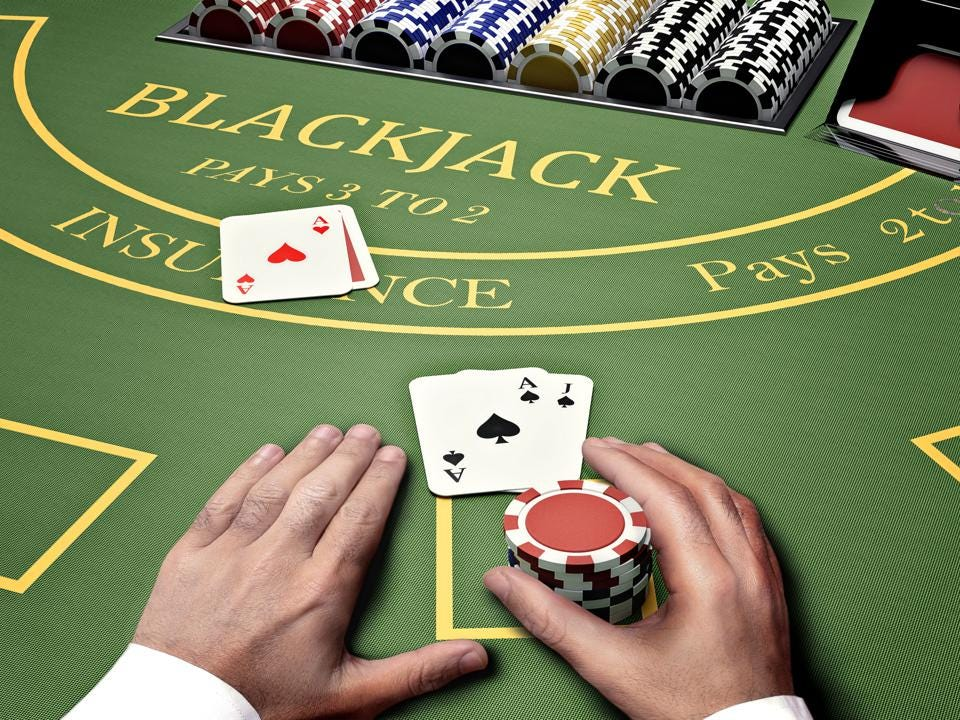
\includegraphics[scale=0.25]{fotos/bl.jpg}
\caption{Foto ilustrativa do Blackjack 21}\cite{blackcapa} %citar local da foto
\end{figure}
Não se sabe ao certo a real origem do BlackJack, porém acredita-se que tenha sido inventado na Espanha. A primeira referência escrita encontra-se num livro do autor espanhol Miguel de Cervantes. Cervantes era um jogador, e os protagonistas de \hyperlink{Glossário}{\textbf{"Rinconete y Cortadillo"}}, são jogadores desonestos em Sevilha. Estes são fraudulentos profissionais em “veintiuna” (espanhol para "vinte e um") que posteriormente viria a ser conhecido como Blackjack. Para além disso afirmam que o objetivo do jogo é chegar a 21 pontos sem ultrapassar.

\hyperlink{Glossário}{\textbf{"Rinconete y Cortadillo"}} foi escrito entre 1601 e 1602, sugerindo que a “ventiuna” era tocada em Castela desde o início do século XVII ou antes. Referências posteriores a este jogo são encontradas na França e na Espanha.
 
O primeiro registo do jogo na França ocorreu em 1888 e na Grã-Bretanha durante as décadas de 1770 e 1780, mas as primeiras regras apareceram na Grã-Bretanha em 1800. \hyperlink{Glossário}{\textbf{Twenty-One}}, ainda conhecido como Vingt-Un, apareceu nos Estados Unidos no início do século XIX. As primeiras regras americanas foram uma reimpressão de 1825 das regras inglesas de 1800. O Vingt-Un inglês mais tarde se desenvolveu em uma variante americana por si só, que foi renomeada como blackjack por volta de 1899.
 
De acordo com o mito popular, quando o Vingt-Un foi introduzido nos Estados Unidos, os locais de jogo ofereciam pagamentos de bónus para aumentar o interesse dos jogadores no Vingt-Un. Um desses bónus era um pagamento de dez para um se a mão do jogador consistisse em um "Ás" de espadas e um valete preto (o valete de paus ou o valete de espadas). Essa mão foi chamada de "blackjack" e o nome continuou mesmo após a remoção desse bónus.
 
Em setembro de 1956, Roger Baldwin, Wilbert Cantey, Herbert Maisel e James McDermott (também conhecidos como 3 dos 4 “Cavaleiros de Aberdeen”), publicaram um artigo intitulado “The Optimum Strategy in Blackjack” no jornal da associação de estatística americana, a primeira estratégia ótima de blackjack matematicamente sólida. Este documento tornou-se a base de futuros esforços para vencer o blackjack. Ed Thorp usou os cálculos da mão de Baldwin para verificar a estratégia básica e posteriormente publicou (em 1963) 
\hyperlink{Glossário}{\textbf{"Beat the Dealer"}}\cite{rules}


\chapter{Regras do jogo}
\label{chap.Regras do jogo}
Em uma mesa de blackjack, o \hyperlink{Glossário}{\textbf{dealer}} enfrenta de cinco a nove posições de jogo atrás de uma mesa em forma de meia-lua. São necessários entre um e oito baralhos padrão de 52 cartas que vão ser baralhados juntos. Para iniciar cada rodada, os jogadores fazem apostas no local ao qual têm direito a colocar as suas fichas, a chamada “caixa de apostas”. Em jurisdições que permitem apostas a favor, é permitido somente até 3 jogadores estarem nas suas respetivas posições. O jogador cuja aposta está na frente da caixa de apostas controla a posição, e o dealer consulta o jogador controlador para decisões de jogo; os outros apostadores "jogam atrás". Um jogador geralmente pode controlar ou apostar em quantas caixas desejar em uma única mesa, porém um indivíduo não pode jogar em mais de uma mesa ao mesmo tempo ou fazer apostas múltiplas em uma única caixa.
 
O dealer negocia da esquerda para a extrema direita, em outras palavras, da ("primeira base") para ("terceira base"). Cada caixa recebe uma mão inicial de duas cartas visíveis para as pessoas que jogam nela. A mão do dealer recebe sua primeira carta virada para cima e, em jogos \hyperlink{Glossário}{\textbf{"hole card"}}, imediatamente obtém uma segunda carta virada para baixo, que o dealer espia, mas só revela quando faz da mão do dealer um blackjack. Às vezes, os jogos de cartas hole são jogados em mesas com algumas medidas de segurança, por exemplo um pequeno espelho ou sensor eletrónico usado para espiar com segurança a carta hole. Nos casinos europeus, prevalecem os jogos "no hole card", por esses motivos.
 
Os dealers distribuem as cartas de um ou dois baralhos de mão, do sapato do dealer ou de uma máquina de embaralhar. As cartas individuais são distribuídas para cada posição apostada no sentido horário, a partir da esquerda do dealer, para além de uma única carta para o mesmo. Posteriormente é fornecida uma carta adicional para cada uma das posições em jogo. As cartas iniciais dos jogadores podem ser viradas para cima ou para baixo.
 
O objetivo do jogo é ganhar dinheiro criando valores totais de cartas maiores que os da mão do dealer, com a condição de não exceder 21, ou parando em um total na esperança de que o dealer estoure. Na sua vez, os jogadores escolhem \hyperlink{Decisões do jogador}{\textbf{"hit"}}, \hyperlink{Decisões do jogador}{\textbf{"stand"}}, \hyperlink{Decisões do jogador}{\textbf{"double"}}, \hyperlink{Decisões do jogador}{\textbf{"split"}} ou \hyperlink{Decisões do jogador}{\textbf{"surrender"}} com os respetivos sinais.
 
As cartas com figuras, ou seja, o rei, a dama e valete têm um valor de 10, as cartas numéricas contam como seu número e os ases ou contam como 1 ou como 11, dependendo da respetiva escolha do jogador. Se o total exceder 21 pontos, ele rebenta e todas as apostas perdem imediatamente.
 
O dealer nunca dobra, divide ou desiste. Se o dealer estourar, todas as mãos restantes do jogador ganham. Se o dealer não estourar, cada aposta restante ganha se sua mão for maior que a do dealer e perde se for menor.
 
Caso um jogador consiga garantir um 21 nas duas primeiras cartas (Exemplo: Valete e Ás) chamado de "natural" ou "blackjack", o jogador ganha imediatamente, a menos que o dealer também tenha um, caso em que a mão empata. Em caso de empate ("push") as apostas são devolvidas sem ajuste. Um blackjack vence qualquer mão que não seja um blackjack, mesmo uma com o valor de 21.
 
As vitórias são pagas com dinheiro igual, exceto para blackjacks de jogadores, que são tradicionalmente pagos com probabilidades de 3 para 2, ou 150\%. Muitos casinos hoje pagam blackjacks em menos de 3:2. Isso é comum em jogos de blackjack de um baralho.


\section{Decisões do jogador}
Esta secção tem como objetivo apresentar as decisões do jogador, juntamente dos respetivos sinais a realizar.
\begin{itemize}
    \item \hypertarget{Decisões do jogador}{\textbf{Hit:} Pegar em outra carta.} \newline
\newline \textbf{Sinal:} Esfregar as cartas na mesa (em jogos portáteis); bater na mesa com um dedo ou acenar com a mão em direção ao corpo (em jogos com a face para cima).
    \item \hypertarget{Decisões do jogador}{\textbf{Stand:} Não pegar em mais cartas; também conhecido como "stand pat", "sit", "stick" ou "stay".} \newline
\newline \textbf{Sinal:} Deslizar os cartões sob os chips (em jogos portáteis); acenar com a mão horizontalmente (em jogos com a face para cima).
    \item \hypertarget{Decisões do jogador}{\textbf{Double:} Aumentar a aposta inicial em 100\% e pegar exatamente mais uma carta. A aposta adicional é colocada ao lado da aposta original. Alguns jogos permitem que o jogador aumente a aposta em valores menores que 100\%, o que é conhecido como "dobrar por menos". Os jogadores que não controlam podem ou não dobrar sua aposta, mas ainda recebem apenas uma carta.} \newline
\newline \textbf{Sinal:} Colocar fichas adicionais ao lado da aposta original fora da caixa de apostas e aponte com um dedo.
    \item \hypertarget{Decisões do jogador}{\textbf{Split:} Criar duas mãos a partir de uma mão inicial em que ambas as cartas tenham o mesmo valor. Cada nova mão recebe outra carta para que o jogador tenha duas mãos iniciais. Isso requer uma aposta adicional na segunda mão. As duas mãos são jogadas independentemente e a aposta em cada mão é ganha ou perdida independentemente. No caso de cartas que valem 10 pontos, alguns casinos só permitem a divisão quando as cartas têm o mesmo valor. A duplicação e a divisão após a distribuição são frequentemente restritas. Uma carta de valor 10 e um "Ás" resultante de uma divisão geralmente não é considerada um blackjack. Acertar ases divididos geralmente não é permitido. Os jogadores que não controlam podem optar por fazer uma segunda aposta ou não. Caso contrário, eles serão pagos apenas ou perderão em uma das duas mãos pós-divisão.}\newline
\newline \textbf{Sinal:} Colocar fichas adicionais ao lado da aposta original fora da caixa de apostas e apontar com dois dedos abertos em uma formação em V.
    \item \hypertarget{Decisões do jogador}{\textbf{Surrender:} Perde metade da aposta e termina a mão imediatamente. Esta opção está disponível apenas em algumas mesas de alguns casinos, e a opção está disponível apenas como primeira decisão.}\newline
\newline \textbf{Sinal:} Falado; não há sinais padrão.\newline
\end{itemize} 


Os sinais manuais ajudam o \hyperlink{Glossário}{\textbf{"olho no céu"}} a fazer uma gravação em vídeo da mesa, que resolve disputas e identifica erros do dealer. Também é usado para proteger o casino contra jogadores desonestos que burlam, ou dealers que roubam fichas. As gravações também podem identificar jogadores de vantagem. Quando o sinal de mão de um jogador discorda de suas palavras, o sinal de mão tem precedência.

Uma mão pode ir buscar uma carta quantas vezes desejar até que o total seja 21 ou mais. Os jogadores devem ficar em um total de 21. Depois que a última mão é jogada, o dealer revela a carta da mão e fica de pé ou empata de acordo com as regras do jogo. Quando o resultado da mão do dealer é estabelecido, todas as mãos com apostas restantes na mesa são resolvidas (geralmente no sentido anti-horário); as apostas em mãos perdedoras são perdidas, a aposta em um empate é deixada na mesa e os vencedores recebem o respetivo pagamento.\cite{rules}






\chapter{Enquadramento teórico}
\label{chap.Enquadramento teórico}
Esta secção tem como objetivo enumerar os diversos conhecimentos necessários para a resolução deste problema. Nomeadamente, na área da programação, é usufruída a Linguagem C para a formulação de um simulador de probabilidades que verifica os resultados teóricos obtidos. Por outro lado, na área da matemática, são utilizadas as teorias da Lei de Laplace, da Probabilidade Condicionada e da Lei dos Grandes Números.

\section{Noções básicas de C}
Criada pelo cientista da computação Dennis Ritchie, em 1972, a linguagem C teve como propósito exclusivo de ser usada no desenvolvimento de uma nova versão do sistema operacional Unix, no entanto, hoje é aplicada nos mais variados tipos de projeto.
\subsection{Estruturas de Decisão}
A cláusula “if” é uma estrutura de decisão que permite estabelecer um controle de fluxo no programa, de forma que o mesmo possa escolher quando executar um determinado bloco de instruções ou não, ou ainda, optar por executar um bloco de instruções em vez de outro \cite{manual}.

\subsection{Estruturas Repetitivas}
A estrutura de decisão “for” é muito útil quando se deseja repetir uma ou várias instruções por um número n de vezes. O comando “while”, não muito diferente do “for”, é geralmente empregado quando não se pode determinar com certeza quantas vezes um bloco de comandos será executado. Em ambos, o objetivo é manter a execução de um bloco de instruções em execução.\\
\subsection{Arrays}
Um array é um conjunto de variáveis do mesmo tipo que podem ser referenciadas por um identificador comum. Em C um array consiste num conjunto de posições de memória contíguas, o qual tem como primeiro índice 0 \cite{silva}.
%\subsection{Utilização de acrónimos}
%Esta é a primeira invocação do acrónimo \ac{om}.
%E esta é a segunda \ac{hd}.

%Outra referência à \ac{om}.

\section{Probabilidades}

\subsection{Lei de Laplace}
No início do século XIX, foi conhecida a primeira definição de probabilidade proveniente do matemático Laplace, aplicando-se apenas para a hipótese de casos equiprováveis e elementares. Portanto, seja A um acontecimento aleatório, pertencente a um conjunto finito E, a sua probabilidade é calculada através da seguinte fórmula:
\begin{equation} \label{eq1}
P(A)=\frac{número de casos favoráveis}{número de casos possíveis}
\end{equation}

\subsection{Probabilidade Condicionada}
Dada uma probabilidade P e dois acontecimentos aleatórios A e B, associados à mesma experiência aleatória, a probabilidade de ocorrer A sabendo que B ocorreu, dá-se pela seguinte fórmula:
\begin{equation} \label{eq2}
P(A\textpipe B)=\frac{P(A\cap B)}{P(B)}
\end{equation}
\subsection{Lei dos Grandes Números}
A Lei dos Grandes Números, formulada pelo matemático Jacob Bernoulli, relaciona o conceito frequencista de probabilidade com o conceito clássico de probabilidade. Isto é, tendo cada experiência um resultado aleatório, a frequência relativa de cada um desses resultados tende a convergir para um certo número teórico, quanto maior for o número de experiências realizadas. Segundo a fórmula apresentada a seguir, a probabilidade de um acontecimento A é igual ao valor do limite do quociente entre o número de casos em que se verifica o acontecimento(Na), e o número de simulações realizadas(N), quando este tende para a frequência do mesmo. \cite{Info}  
\begin{equation} \label{eq3}
P(A)= \lim_{x \rightarrow +\infty} \frac{Na}{N}
\end{equation}
\newpage
\section{Blackjack 21}
Como foi mencionado no capitulo anterior (\autoref{chap.Regras do jogo}), o blackjack trata-se de um jogo de cartas que pode conter 1 a 8 baralhos de 52 cartas, em que o objetivo é ter mais pontos do que o adversário, sem ultrapassar no entanto os 21 pontos (caso aconteça, esse jogador perde). O dealer/crupiê (profissional responsável pela mesa) só pode pedir até um máximo de 5 cartas ou até chegar ao número 17. Na tabela que se segue, são apresentados os valores correspondentes a cada carta,destacando-se o facto de a carta "Ás" possuir diferentes valores consoante a restante carta c mão \cite{cardoso2018estudo}.
\begin{figure}[H]
\center
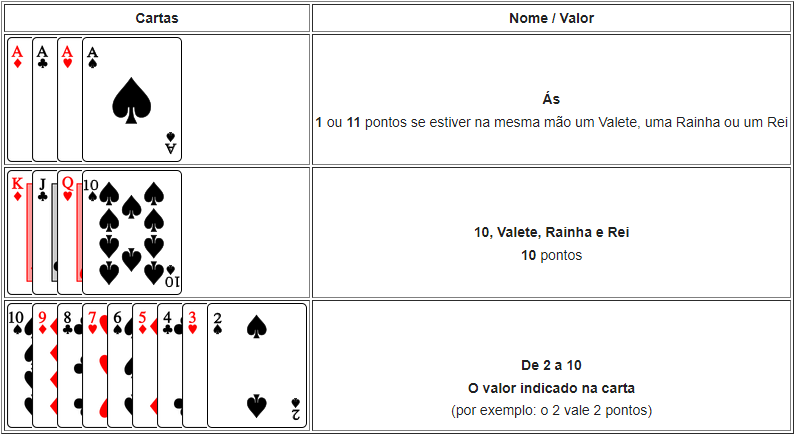
\includegraphics[scale=0.36]{fotos/3.png}
\caption{Pontuação das cartas Blackjack \cite{wiki}}
\end{figure}
\chapter{Questão de investigação}
\label{chap.Questão de investigação}
Através da realização deste relatório, pretende-se responder à seguinte questão: A partir de quantas experiências/jogadas se verifica a probabilidade teórica de saírem exatamente 21 pontos? 

\chapter{Metodologia}
\label{chap.Metodologia}
Na procura de uma resposta à questão anteriormente mencionada começou-se por calcular as probabilidades matemáticas de sair exatamente 21 pontos em diferentes mãos/jogadas, que resultarão no valor teórico. De seguida, e por outro lado, procedeu-se ao desenvolvimento de um código em C com o intuito de simular um "n" número de jogadas. Por último, pretende-se verificar ao fim de quantas jogadas o valor experimental se aproxima do valor teórico (calculado anteriormente), segundo a Lei dos Grandes Números.

\chapter{Desenvolvimento}
\label{chap.Desenvolvimento}
Nesta secção é apresentada, primeiramente, o cálculo matemático da probabilidade teórica e de seguida, é ilustrado e explicado o procedimento da construção de um programa simulador que visa a prever a probabilidade experimental. No tópico "Discussão dos Resultados" será verificado ao fim de quantas simulações feitas pelo programa o valor da probabilidade experimental irá aproximar-se da probabilidade teórica.\\\textbf{Nota:} De forma a limitar a complexidade do problema, assumiu-se que a carta "Ás" terá um único valor(11).

\section{Probabilidade Teórica}
No cálculo da probabilidade teórica utilizou-se a primeira definição de probabilidade "Lei de Laplace". Posto isto, enumerou-se todas as combinações possíveis para fazer 21 pontos com duas, três, quatro ou cinco cartas na mão, multiplicou-se pelos 4 naipes e chegou-se a um valor de 445830 jogadas favoráveis. De seguida, dividiu-se este número pelo número total de jogadas possíveis neste jogo chegando-se ao valor de 0.1541.

\begin{equation} \label{eq4}
P(A)=\frac{Casos favoráveis}{Casos possíveis}
\end{equation}
\centerline{$\Leftrightarrow P(A)=\frac{445830}{C_2^5^2+C_3^5^2+C_4^5^2+C_5^5^2}$}
\\\\ \centerline{$\Leftrightarrow 
P(A)\backsimeq0,1541$}
\newpage
\section{Programa}
Inicialmente, para a construção do programa em linguagem C, começa-se por indicar as seguintes variáveis:
\begin{scriptsize}
\estiloJava
\begin{lstlisting}
int flag;     
int valor;  
\end{lstlisting}
\end{scriptsize}
"flag" que tem como objetivo verificar se a carta já foi usada ou não; "valor" que apresenta a função de atribuir o valor da carta.\\
\\Seguidamente cria-se uma função "config" onde se configura o valor de cada carta.
\begin{scriptsize}
\estiloJava
\begin{lstlisting}
void config(Cartas* baralho) {  
    int aux=2;
    for (int i=0; i<52; i++) {      
        if (aux==12) aux=2;         
        baralho[i].valor=aux;
        if (aux==10) {
            baralho[i+1].valor=aux;
            baralho[i+2].valor=aux;
            baralho[i+3].valor=aux;
            i=i+3;
        }
        aux++;
\end{lstlisting}
\end{scriptsize}
Posteriormente, cria-se uma função "baralhar", que tal como o nome indica, pretende embaralhar as cartas, ou seja, colocá-las como não usadas.
\begin{scriptsize}
\estiloJava
\begin{lstlisting}
void baralhar(Cartas* baralho) {    
    for (int i=0; i<52; i++) {          
        baralho[i].flag=0;
    }
\end{lstlisting}
\end{scriptsize}
\newpage
Cada carta corresponde a uma variável do array "baralho", de índice 0 a 51, tal como observamos nesta figura.
\begin{figure}[H]
\center
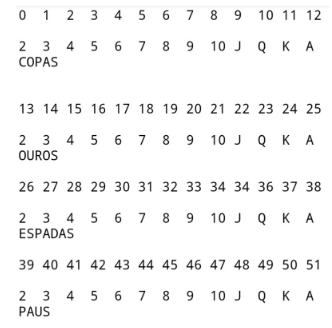
\includegraphics[scale=0.7]{fotos/2.png}
\caption{Cartas correspondentes às variáveis do array \cite{paper}}
\end{figure}
Geram-se novas variáveis, respetivamente: número de jogadas; pontuação que se acumula ao longo da jogada; limite de cartas retiradas; carta retirada; número de BlackJacks; probabilidade experimental.
\begin{scriptsize}
\estiloJava
\begin{lstlisting}
long double num_jogadas; 
    int pontuacao=0, pontuacao2=0;   
    int lim=0;                      
    int x;                              
    int nBJ=0;                          
    double probabilidade;
\end{lstlisting}
\end{scriptsize}
Foi introduzida uma estrutura de repetição que pretende criar um ciclo finito onde é perguntado ao utilizador o número de simulações que quer realizar.\\
\\De seguida, é criada uma função "GerarMao()", em que é gerado um número "random" de 0 a 51, x, e, aplicando uma estrutura de decisão, verifica-se se a carta já foi usada e consecutivamente marcá-la como usada.
\begin{scriptsize}
\estiloJava
\begin{lstlisting}
for (int i=0; i<num_jogadas; i++) {         
        baralhar(baralho);
        pontuacao=0; pontuacao2=0; lim=0;
        while(pontuacao<=21 && pontuacao2<=21 && lim<6) {
            x = rand()% 52;                        
            if (baralho[x].flag==0) {               
                lim++;
                baralho[x].flag=1;                  
                pontuacao += baralho[x].valor;
            }
\end{lstlisting}
\end{scriptsize}
\newpage
Depois, formou-se uma nova estrutura de decisão para verificar se atingiu-se os exatos 21 pontos em alguma das jogadas. 
\begin{scriptsize}
\estiloJava
\begin{lstlisting}
if (pontuacao==21 || pontuacao2==21) {  
                nBJ++;
            }
\end{lstlisting}
\end{scriptsize}
Por fim, é calculada e exposta a probabilidade de fazer um blackjack consoante o número de jogadas requeridas pelo utilizador.
\begin{scriptsize}
\estiloJava
\begin{lstlisting}
probabilidade = ((double)nBJ/(double)num_jogadas)*100; 

printf("Numero de BlackJacks = %d\n", nBJ);          
printf("Probabilidade = %lf\n", probabilidade);
\end{lstlisting}
\end{scriptsize}
\newpage
\section{Discussão dos resultados}
Após a concretização do programa, simulou-se a probabilidade experimental para nove números de jogadas distintas. De forma a obter probabilidades experimentais mais precisas, foram realizadas cinco repetições para o mesmo número de jogadas e posteriormente efetuada a média dessas mesmas cinco repetições.\
\begin{table}[ht]
\centering
\begin{tabular}{c c}
\hline
Nº de Jogadas & Probabilidade(\%) \\ [0.5ex] % inserts table %heading
\hline
10&18.0000\\[1ex]
10^2&15.8000\\[1ex]
10^3&14.7400\\[1ex]
10^4&15.6480\\[1ex]
10^5&15.3674\\[1ex]
10^6&15.4246\\[1ex]
10^7&15.412150\\[1ex]
10^8&15.4117735333\\[1ex]
10^9&15.41065728333\\
\hline
\end{tabular}
\caption{Variação do valor das probabilidades em função do número de jogadas}
\label{tab:my_label}
\end{table}

Os dados da tabela expostos anteriormente foram inseridos num gráfico de forma a estudar a linha de tendência.
\begin{figure}[H]
\center
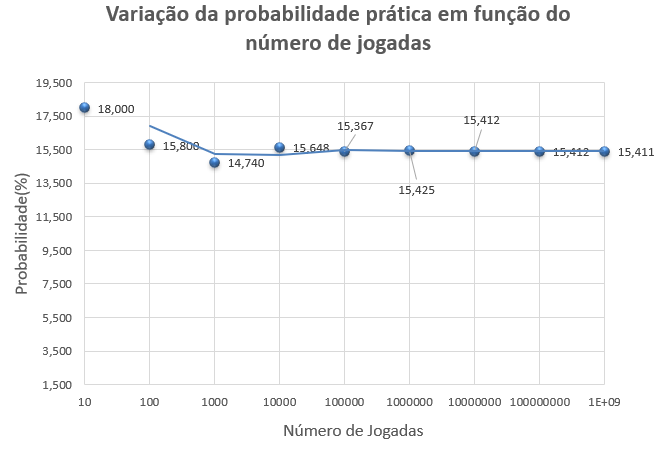
\includegraphics[scale=0.45]{fotos/1.png}
\caption{Probabilidade de sair 21 pontos no BJ em função do número de jogadas}
\end{figure}

Após a observação do gráfico é percetível de que a linha tende para um certo valor. Portanto, chega-se à conclusão de que a probabilidade experimental de fazer 21 pontos no Blackjack é 15.412\%.

\chapter{Conclusão}
\label{chap.conclusao}
Após toda a realização do desenvolvimento, concluí-se primeiramente que para o valor experimental se aproximar verdadeiramente do valor teórico são necessárias um número muito elevado de simulações. Neste caso em particular, foram precisas cerca de dez milhões de jogadas para se verificar a "Lei dos Grandes Números". Concluí-se também que a probabilidade de fazer 21 pontos num jogo de blackjack é aproximadamente 15,41\%. Contudo, é de real importância destacar de novo que o valor da carta "Ás", ao longo do desenvolvimento, tomou unicamente o valor de 11 pontos, algo que poderia ser acrescentado a este problema em específico, com o objetivo de ampliar o âmbito deste trabalho.

% \chapter{Referências bibliográficas}
% \label{chap.Referências bibliograficas}

\chapter*{Contribuições dos autores}

Os dois cooperamos de forma igual na realização do projeto. Dividimos e estabelecemos no inicio do trabalho o que cada um ficava responsável por realizar. \newline

O aluno \ac{om} ficou responsável pela pesquisa de todo o capítulo do Enquadramento Teórico para além da parte referente à programação e teste do simulador que calcula a probabilidade. \newline

O aluno \ac{hd} pesquisou acerca da história do blackjack e as respetivas regras. \newline

Ambos contribuíram no desenvolvimento da estrutura do projeto \LaTeX \newline

Orlando Marinheiro - \ac{om}
Hugo Dias - \ac{hd}
\vspace{10pt}
%\textbf{Indicar a percentagem de contribuição de cada autor.}\\

\autores : 50\%, 50\%\\

%%%%%%%%%%%%%%%%%%%%%%%%%%%%%%%%%
\chapter*{Acrónimos}
\begin{acronym}
\acro{om}[OM]{Orlando Marinheiro}
\acro{hd}[HD]{Hugo Dias}
\acro{glisc}[GLISC]{Grey Literature International Steering Committee}
\end{acronym}

\chapter*{Glossário}

\hypertarget{Glossário}{\textbf{Beat the Dealer:} O livro que fez Las Vegas mudar as regras. Edward O. Thorp é o pai da contagem de cartas e, neste guia clássico, ele compartilha o revolucionário sistema de pontos que tem sido usado com sucesso por jogadores de cartas profissionais e amadores por gerações.
Foram impressas mais de 1.000.000 de cópias.}
\newline
\paragraph{}\hypertarget{Glossário}{\textbf{Rinconete y Cortadillo:} "Rinconete y Cortadillo" é um conto entre os doze contos incluídos em “Novelas Exemplares”, do escritor espanhol Miguel de Cervantes.}
\paragraph{}\hypertarget{Glossário}{\textbf{Dealer:} Jogador que distribui as cartas durante o jogo.}
\newline
\paragraph{}\hypertarget{Glossário}{\textbf{Hole card:} Uma carta de baralho, virada para baixo, que o dealer não precisa revelar até à hora de decidir a jogada.}
\newline
\paragraph{}\hypertarget{Glossário}{\textbf{ Twenty-One:} Twenty-One, anteriormente conhecido como vingt-un na Grã-Bretanha, França e América, é o nome dado a uma família de jogos de cartas populares da família do jogo, cujo progenitor está registado na Espanha no início do século XVII.}
\newline
\paragraph{}\hypertarget{Glossário}{\textbf{Olho no céu:} O olho no céu é um termo dado a casinos e outras câmaras de circuito fechado de segurança comercial. Nos casinos, eles estão posicionados para monitorizar assentos, mesas, corredores, restaurantes e até mesmo elevadores de perto. O componente funcional é conhecido como câmara pan-tilt-zoom, ou PTZ, um termo padrão da indústria.}
\newline

%%%%%%%%%%%%%%%%%%%%%%%%%%%%%%%%%
\printbibliography
\end{document}
